\section{The Algorithm}
\label{S:Alg}

\subsection{Overview}
\label{SS:Alg:Overview} 


Howard's multi-robot SLAM algorithm generates a single map and pose posterior much in the same way an occupancy grid map SLAM algorithm based on a Rao-Blackwellized particle filter (RBPF) would, but with additions to accommodate multiple robots. Mapping begins with a set consisting of a single robot with known pose and an occupancy grid map of the environment is built as this robot traverses and measures it. The ultimate goal of the algorithm is to simultaneously compute for time $t$, the full SLAM posterior containing all robot pose trajectories $x_{1:t}^i$ and the global map $m_{1:t}$, given only a single known initial pose and sets of measurements
\begin{align*}
p(x_{1:t}^1,x_{1:t}^2&,...,x_{1:t}^M,m_{1:t}|\\&x_0^1,z_{1:t}^1,u_{0:t}^1,\Delta_s^2,z_{1:t}^2,u_{0:t}^2,\Delta_s^3,...,\Delta_s^M,z_{1:t}^M,u_{0:t}^M)
\end{align*}

The odometry and measurement data of all other robots is stored as it is collected, as it cannot contribute to the global map without a known relative pose linking it to the frame of the first robot. As the first robot encounters additional robots via a mutual pose observation, the newly observed robot is added to the set of mapping robots and its actions and the map is sequentially conditioned by its actions and measurements. From the point of observation, all future actions and measurements of the new robot are used to condition the map posterior, and likewise all of its previously stored actions and measurements are played back in reverse order from that point as a virtual robot. This information is then passed to a pair of new particle filters for the pose of these robots that contribute to the same global map. Figure \ref{fig:forwardbackward} gives a graphical example of an encounter where a causal and acausal virtual robot are spawned from a robot encounter.
\begin{figure}[ht]
\centering
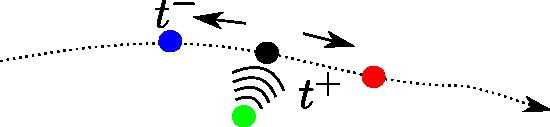
\includegraphics[width=\columnwidth]{../FinalFigures/ForwardBackward.pdf}
\caption{Causal and Acausal Virtual Robots Added on Encounter}
\label{fig:forwardbackward}
\end{figure}

As further encounters occur between any robot, real or virtual, in the mapping set and a previously unseen robot, the previously unseen robot is added to the set of mapping robots and its measured relative pose is again used to establish a reference point with which its actions and measurements can condition the map posterior. Further mutual observations of two robots already in the mapping set are ignored for the sake of simplicity. This encounter-add process is continued recursively for all robots until all stored and future odometry and measurements are exhausted or all possible mapping robots have made an encounter with the mapping set. Beyond this point, the algorithm behaves as a normal RBPF with a stacked state containing pose posteriors of all robots in addition to the map.


This algorithm relies on a number of assumptions that are requisite for it to effectively solve the MRSLAM problem. Firstly, for all explored regions to count towards the map, each mapping robot must have encountered a robot that is an element of the mapping set in order to make a fully connected graph of robot poses, and therefore maximally complete map. Additionally, each robot pose trajectory is independent of all other trajectories such that motion or observation from one robot does not affect another outside of encounter events \cite{howard2006multi}.

\subsection{Algorithm Details}
\label{SS:Alg:Details}
Our implementation of Howard's MRSLAM algorithm follows the basic structure of the below steps that perform data queueing, robot encounter management, and FastSLAM filter updates.
\begin{enumerate}
\item Queue measurement, odometry, and mutual observation (encounter) data
\item For all robots in the mapping set, take first element from queue and update SLAM filter
\item For all new encounters, split encountered queue at present time into causal and acausal queues and instantiate a new set of particles for the causal and acausal trajectory of the observed robot.
\item For all available acausal queues, remove last element and use it to update the SLAM filter for the corresponding acausal robot
\item If data includes a prior encounter with a robot not in the mapping set, instantiate a new set of particle for this robot and its acausal virtual self at its location and split the queue for that robot into a causal and acausal queues
\item Resample all particles to prevent weighting degeneracy
\item Repeat until all data is consumed
\end{enumerate}
\vspace{0.1in}
\subsubsection{Data Queueing}
As each robot $R$ collects data, its current odometry $u_t^R$ and measurements $z_t^R$ are added to a running queue data structure before processing. An encounter flag $E_t^R$ and relative pose $\Delta_t^R$, if available, are also added to this queue. 
$$queue_{0:t}^R = append(queue_{0:t-1}^R, \{ u_t^R, z_t^R, E_t^R, \Delta_t^R \})$$
The storing of this data allows for either immediate use by particle filters for robots in the mapping set, or later joining or SLAM filtering after a future encounter with a mapping robot.
\vspace{0.1in}
\subsubsection{Encounters}
An encounter in this sense is defined as the observation of one robot by another mapping robot that produces a relative pose estimate between the robots of $\Delta$. For this implementation, it was assumed that the estimation of $\Delta$ was deterministic for the sake of demonstration and simplicity.

Upon an encounter at time $s$ between robot $A$ in the mapping set with a pose $x_s^A$ and a robot $B$ not in the set with a measured relative pose $\Delta_s^{AB}$, a reference frame pose for each particle $i$ of the newly observed robot is instantiated as causal particle posterior $x_s^{B(i)}$ and acausal particle pose posterior $\bar{x}_s^{B(i)}$ as:
\begin{align*}
x_s^{B(i)} &= x_s^{A(i)} \oplus \Delta_s^{AB} \\
\bar{x}_s^{B(i)} &= x_s^{A(i)} \oplus \Delta_s^{AB}
\end{align*}
Where $\oplus$ is the pose composition operator. <SSC reference?>
At this time, the stored data queue for robot B is also split into a causal queue $queue^B$ and acausal queue $\bar{queue}^B$.
\begin{align*}
\bar{queue_{t+1:}^B} = reverse(queue_{0:t-1}^B) \\
queue^B = queue_{t+1:}^B
\end{align*}

If neither robot is within the mapping set and an encounter occurs, this encounter and the associated measured relative pose is stored for later use. In the event that one of these robots later encounters a robot in the mapping set, its virtual acausal robot will spawn another robot pair of the unencountered robot upon backtracking to the location of this initial encounter. At this acausal encounter, the same method of adding relative pose and splitting the queues used in the causal join is used to generate the causal and acausal virtual robots created by this encounter.

Figure \ref{fig:multiencounter} explains the joining process graphically. The scenario starts with three robots $x^1$, $x^2$, and $x^3$, with $x^1$ being the sole robot in the initial mapping set. The actual robots are represented as white circles, the causal particles as red circles, the acausal particles as blue circles, and encounters as purple arrows. At timestep $T_1$, an encounter occurs between $x^2$ and $x^3$, but neither is in the mapping set at this time, so this encounter is stored. At timestep 2, robots $x^1$ and $x^2$ encounter each other, spawning a causal and acausal pair of pose particles $x^{2+}$ and $x^{2-}$ respectively. $x^{1+}$ and $x^{2+}$ continue propagating forward with new data (not shown) while $x^{2-}$ propagates backwards in time using stored odometry and measurements. The stored encounter between $x^2$ and $x^3$ that was previously stored is then incorporated at time $T_3$ when the acausal particles $x^{2-}$ reach the location of the encounter. This spawns a set of particles for the previously encounter robot $x^3$. As the original encounter happened on the first step, no acausal particles are spawned at this time. As $x^{2-}$ reaches the last remaining pose in the acausal queue, the particles are removed as the past data is exhausted.

%\begin{figure}[ht!]
%\centering
	%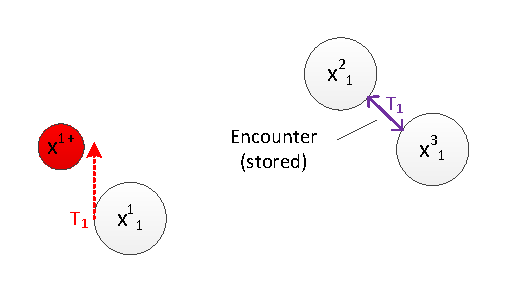
\includegraphics[width=3in]{../FinalFigures/multiencounter_1.pdf} \\
	%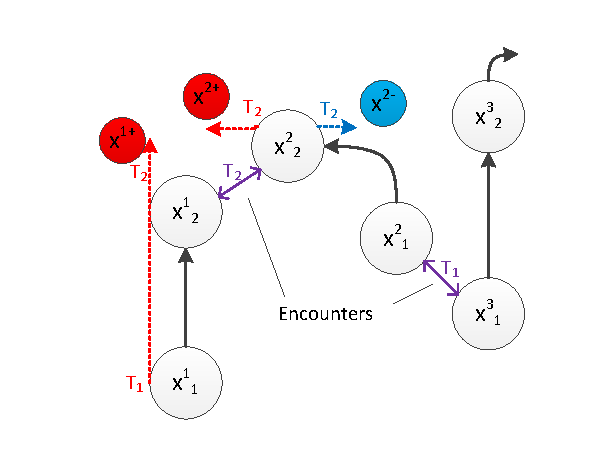
\includegraphics[width=3in]{../FinalFigures/multiencounter_2.pdf} \\
	%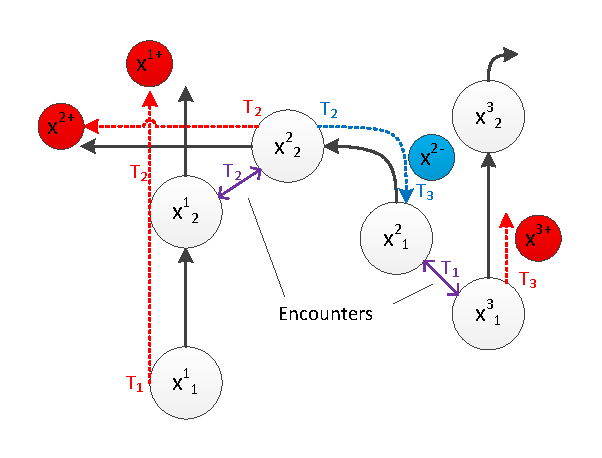
\includegraphics[width=3in]{../FinalFigures/multiencounter_3.pdf} \\
	%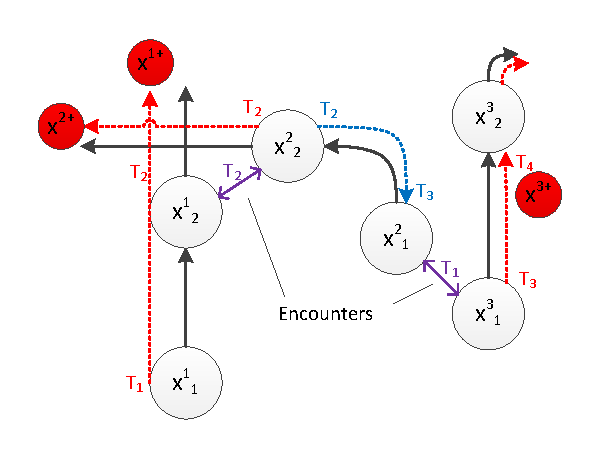
\includegraphics[width=3in]{../FinalFigures/multiencounter_4.pdf} \\
%\caption{Example of Robot Encounters in this MRSLAM Implementation}
%\end{figure}

\newcommand{\codymult}{0.75}
\begin{figure}[ht!]
\centering
    \subfigure[Timstep 1]{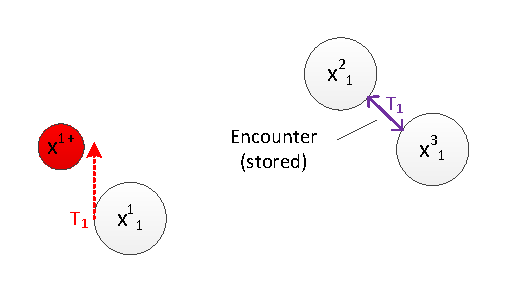
\includegraphics[width=\codymult\columnwidth]{../FinalFigures/multiencounter_1.pdf}} \\
    \subfigure[Timestep 2]{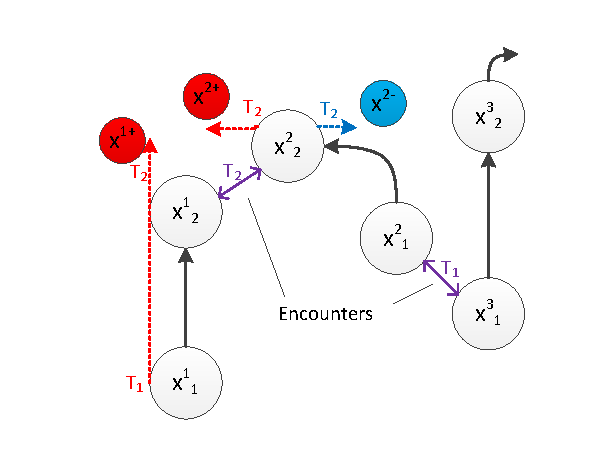
\includegraphics[width=\codymult\columnwidth]{../FinalFigures/multiencounter_2.pdf}} \\
    \subfigure[Timestep 3]{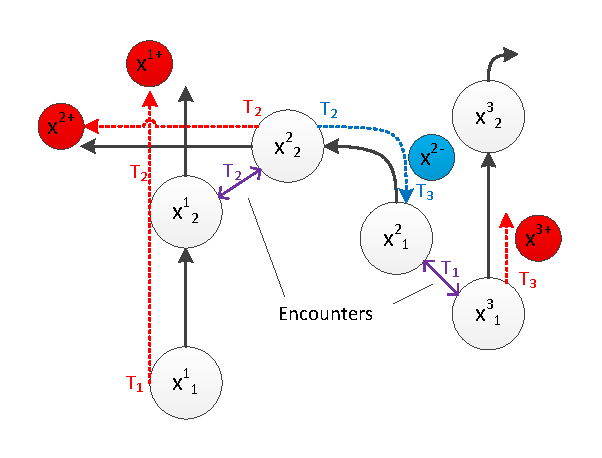
\includegraphics[width=\codymult\columnwidth]{../FinalFigures/multiencounter_3.pdf}} \\
    \subfigure[Timestep 4]{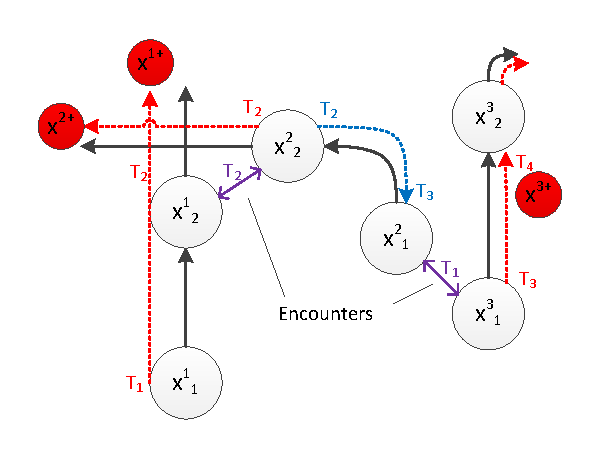
\includegraphics[width=\codymult\columnwidth]{../FinalFigures/multiencounter_4.pdf}} \\
\caption{Example of Robot Encounters in this MRSLAM Implementation}
\label{fig:multiencounter}
\end{figure}

\vspace{0.1in}
\subsubsection{FastSLAM Updates}
At each time-step, the pose posterior is updated for all pose states within the current mapping set are updated according to a modified Rao-Blackwellized particle filter. Both information from the causal and acausal queues is used to update the SLAM posterior in an almost identical fashion, save for a time-reversed odometry model. 

This process first applies an odometry prediction to each particle. This single update applies to each causal robot particle a forward odometry change given an arbitrary non-linear and noisy forward odometry model $g(x,u)$. For each virtual robot traversing its path in reverse, the next stored point is popped off the corresponding stack and used with a noisy inverse odometry model $g_r(x,\bar{u})$
\begin{align*}
x_{t+1}^{r(i)} &= g(x_{t}^{r(i)},u_{t+1}^{r(i)})\\
\bar{x}_{t+1}^{r(i)} &= g_r(\bar{x}_t^{r(i)}, \bar{u}_{t+1}^{r(i)})
\end{align*}
The odometry prediction step was followed by an occupancy grid map update for each real or virtual robot particle based on current or stored measurements. For each robot $R$, whether it represents causal or acausal particles, the next measurement in the queue, $z_t^R$ is removed and used to update the map for each particle according to a simplified occupancy grid measurement model.

For each particle in $x_t^R$,  the particle's associated map $m_i$, and associated measurement $z_t^R$ is used with the simplified inverse sensor model to compute the log-odds of a particular cell’s occupancy. Our chosen model simulated a typical range,bearing LIDAR type sensor, with a fixed occupied (black) and free (white) probability and simple sensor cone model similar to the one shown in Figure \ref{fig:invsensor}.

\begin{figure}[ht]
\centering
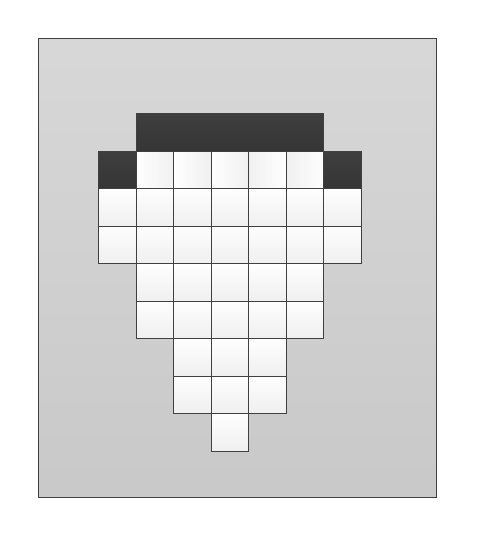
\includegraphics[width=\columnwidth]{../FinalFigures/invsensormodel.pdf}
\caption{Example Inverse Sensor Model Pattern}
\label{fig:invsensor}
\end{figure}

For each cell augmented by the inverse sensor model, the log-odds was updated as:
$$l_{t,i}=l_{t-1,i}+l_{sensor,t,i}-\log\frac{p(m_i)}{1-p(m_i)}$$

After incorporating the the next measurement for all particles to each map particle, the last portion of the SLAM update consists of updating each pose particle’s weight and resampling to prevent weighting degeneracy.

The weighting of each particle in this step was adjusted using the measurement likelihood given the robot's estimated pose and the current map 
$$w^{(i)}=p(z_t^{1(i)}|x_t^{1(i)},m_t)p(z_t^{2(i)}|x_t^{2(i)},m_t)...p(z_t^{M(i)}|x_t^{M(i)},m_t)$$. 

We also implemented an algorithm that assigns an independent particle weighting for each independent pose particle set. For robot R, this weight was computed as:
$$w^{R(i)}=p(z_t^{R(i)}|x_t^{R(i)},m_t)$$

After the propagation and update, the FastSLAM algorithm performs stochastic universal resampling to generate an update set of uniform weight samples. All weights are normalized such that they sum to 1, a cumulative mass function is generated, and a random initial offset is chosen. From this initial offset, an identical number of samples equally spaced across the CMF are taken and the inverse CMF at each of those samples is used to create a new particle. The resulting weights of each particle are then set to a uniform value. 

For our addition where each set of pose particles has independent weights, these weights are used to independently resample each pose set while leaving the map unchanged. Stochastic universal resampling is also used for this process.
\vspace{0.1in}
\subsubsection{Commentary on Sequential Updating}
By only incorporating a fixed number of odometry and measurement updates in a given timestep, Howard's MRSLAM algorithm places a bound on computation time\cite{howard2006multi}. Each particle propagation, and map update, and measurement model weighting computation are constant time operations for a fixed map size. This results in bounds on computational complexity for a fixed map size using $m$ robots each with $n$ particles of $\mathcal{O}(mn)$. Incorporating all past measurements simultaneously would require computing a possibly large number of particle filter updates \cite{howard2006multi}. Using Howard's algorithm, where particle weights are shared across all poses, would also be at risk of resampling impoverishment where existing partcles would die out as a result of a simultaneous incorporation of all acausal data at an encounter.
